\section{Implementation and Prototype}
\label{ch:impl}

This section describes how the design was implemented: the project structure, the back end, the front end and its design system, the pilot dataset, and the traceability from requirements to code.

\subsection{Project Structure and Environment}

The source code is hosted in one Git repository~\cite{chacon2014progit} with three main folders: \code{frontend} (Next.js application), \code{backend} (Express API and SQL schema) and \code{docs} (diagrams, use cases, data dictionary, pilot dataset). Table~\ref{tab:stack} gives the versions and roles of the main tools.

\begin{table}[H]
\centering
\caption{Technology stack and versions}
\label{tab:stack}
\begin{tblr}{colspec={Q[l,3.4cm]Q[l,3.4cm]X[l]}, row{1}={font=\bfseries}, hline{1,Z}={0.8pt}, hline{2}={0.4pt}, rowsep=3pt}
Layer & Technology & Role\\
Front end & Next.js 14.2, React 18.3 & Pages, components, client-side state~\cite{nextjsdocs, reactdocs}\\
Styling & Plain CSS with custom properties & Design tokens, light and dark themes\\
Back end & Node.js, Express 5, TypeScript & REST API~\cite{nodedocs, expressdocs, typescriptdocs}\\
Security libraries & \texttt{bcryptjs}, \texttt{jsonwebtoken} & Password hashing and tokens~\cite{provos1999bcrypt, rfc7519}\\
Database driver & \texttt{pg} & Parameterized SQL\\
Database & PostgreSQL 15, \texttt{pgcrypto} & Storage and integrity~\cite{postgresdocs}\\
Version control & Git & Collaboration of three developers\\
\end{tblr}
\end{table}

\subsection{Back-End Implementation}

\subsubsection{Structure}

The API is organized in the following modules:

\begin{itemize}
    \item \code{config/}: reads environment variables (database URL, JWT secret, port) and creates the connection pool;
    \item \code{middleware/auth.ts}: verifies the JWT and provides \code{requireRoles(...)};
    \item \code{routes/auth.ts} and \code{routes/quizzes.ts}: registration, login and quiz submission;
    \item \code{routes/academic.ts}: schedule, sessions, enrollment, attendance and statistics;
    \item \code{server.ts}: starts the HTTP server and the expiry sweep.
\end{itemize}

\subsubsection{Authentication and Roles}

Registration hashes the password with bcrypt and inserts a student. Login verifies the hash and returns a JWT valid for one day containing the user identifier and role. The middleware \code{requireRoles} receives the list of allowed roles of a route; for example, the opening of attendance is restricted to \code{instructor} and \code{admin}, and the route additionally checks that the instructor owns the class.

\subsubsection{Bulk Creation of Sessions}

The endpoint \code{POST /api/classes/:classId/sessions/bulk} creates sessions 1--15 inside one database transaction. If one session is invalid (for example, its end time is before its start time) the whole request is rolled back, so a class never ends up with a partial timetable. This follows the business rule that a class has exactly fifteen sessions (R5 in Table~\ref{tab:br}).

\subsubsection{PIN Attendance}

Opening the window generates the PIN and the expiry:

\begin{lstlisting}[language=TS, caption={Generation of the PIN (excerpt)}, label={lst:pin}]
import { randomInt, timingSafeEqual } from 'node:crypto'

// 0000 - 9999, uniformly distributed, from a cryptographically secure source
const code = randomInt(0, 10_000).toString().padStart(4, '0')
\end{lstlisting}

The check-in endpoint runs in one transaction and follows the steps below. The listing shows the order of the checks; the HTTP status code of each rejection is given in Table~\ref{tab:checkin}.

\begin{enumerate}
    \item Load the session and verify that the student has an \emph{enrolled} row for its class.
    \item If the window is closed or the expiry has passed, clear the PIN and answer \texttt{410}.
    \item Take a transaction-level advisory lock on the pair (session, student) so that parallel requests of the same student are processed one at a time.
    \item Count the failed attempts of the student for this session in the last 15 minutes; if there are five or more, answer \texttt{429}.
    \item Compare the PIN with \code{timingSafeEqual}. If different, insert a failed attempt and answer \texttt{401}.
    \item Insert the attendance record with \code{ON CONFLICT (session_id, user_id) DO NOTHING}. If nothing was inserted, answer \texttt{409}; otherwise log a successful attempt and answer \texttt{201}.
\end{enumerate}

\begin{table}[H]
\centering
\caption{Outcomes of the check-in endpoint}
\label{tab:checkin}
\begin{tblr}{colspec={Q[l,1.6cm]X[l]}, row{1}={font=\bfseries}, hline{1,Z}={0.8pt}, hline{2}={0.4pt}, rowsep=3pt}
Status & Meaning\\
201 & Check-in recorded. The status is \emph{late} if the check-in time is after the scheduled start of the session in the Asia/Ho\_Chi\_Minh time zone, and \emph{present} otherwise.\\
401 & The PIN is incorrect; a failed attempt is logged.\\
409 & The student already has a record for this session.\\
410 & The window is closed or expired.\\
429 & Five failed attempts in the last 15 minutes.\\
\end{tblr}
\end{table}

A timer started with the server calls a function every 15 seconds that sets \code{attendance_code}, \code{is_attendance_open} and \code{attendance_expires_at} to their closed values for every session whose expiry has passed. The check-in endpoint also tests the expiry itself, so the correctness of the system does not rely on the timer.

\subsubsection{Attendance Rate}

The summary endpoint computes, for each student, the number of attended sessions among the completed ones. A session is \emph{completed} when its scheduled end time (in the Asia/Ho\_Chi\_Minh time zone) has passed. Present and late count as attended, excused sessions are removed from the denominator, and a missing record counts as not attended. The overall rate is the number of attended check-ins divided by the number of expected student--session pairs without excused ones.

\subsubsection{Quiz Submission}

\code{POST /api/quizzes/:quizId/submit} receives the list of answers, loads the answer key on the server, compares, and inserts one \code{quiz_interactions} row per answer with the question, skill, session, correctness and attempt number. The learner-facing quiz endpoint never selects \code{correct_answer}.

\subsection{Front-End Implementation}

\subsubsection{Design System}

The interface is a reproduction of the BKeL portal with a refined design system:

\begin{itemize}
    \item \textbf{Color.} Primary \texttt{\#008299} (BKeL teal) and a neutral scale; semantic colors for present, late, absent and excused. Both themes keep a contrast ratio of at least 4.5:1 for body text.
    \item \textbf{Icons.} 100\% inline SVG in the Moodle style for activity types (PDF, quiz, attendance, code, forum, calendar, timetable). No emoji is used anywhere.
    \item \textbf{Course cards.} Geometric vector patterns (circles, triangles) similar to the Moodle default course images.
    \item \textbf{Motion.} Short transitions (under 400\,ms) for tab changes and modals; the reduced-motion setting of the operating system is respected.
    \item \textbf{Themes.} Light and dark themes by switching CSS variables; the choice is stored in the browser.
\end{itemize}

\subsubsection{Pages}

Table~\ref{tab:pages} lists the pages and tabs of the prototype.

\begin{table}[H]
\centering
\caption{Pages and tabs of the front-end prototype}
\label{tab:pages}
\begin{tblr}{colspec={Q[l,3.4cm]X[l]Q[l,2.4cm]}, row{1}={font=\bfseries}, hline{1,Z}={0.8pt}, hline{2}={0.4pt}, rowsep=3pt}
Page or tab & Content & Use case\\
Login (CAS style) & Separate entry for the lecturer and the student role; sample accounts for demonstration & UC1\\
Home / dashboard / my courses & Course cards for the active semester & UC1\\
Course: Sessions & The 15 sessions with title, date, room and materials & UC5\\
Course: Attendance & Open window with PIN and countdown (lecturer); PIN entry (student); live list & UC6\\
Course: Timetable & Weekly grid with today's session highlighted & UC5\\
Course: Participants & Enrolled students & UC7\\
Course: Statistics & Enrollment against capacity; participation per session; rate per student & UC7\\
Course: Quiz & Question bank of 40 questions; whole-bank quiz or one quiz per session & UC2\\
\end{tblr}
\end{table}

\subsubsection{Screens}

Figures~\ref{fig:login}--\ref{fig:stats} show the main screens. The interface language of the prototype is Vietnamese, in agreement with the users of HCMUT.

\begin{figure}[H]
\centering
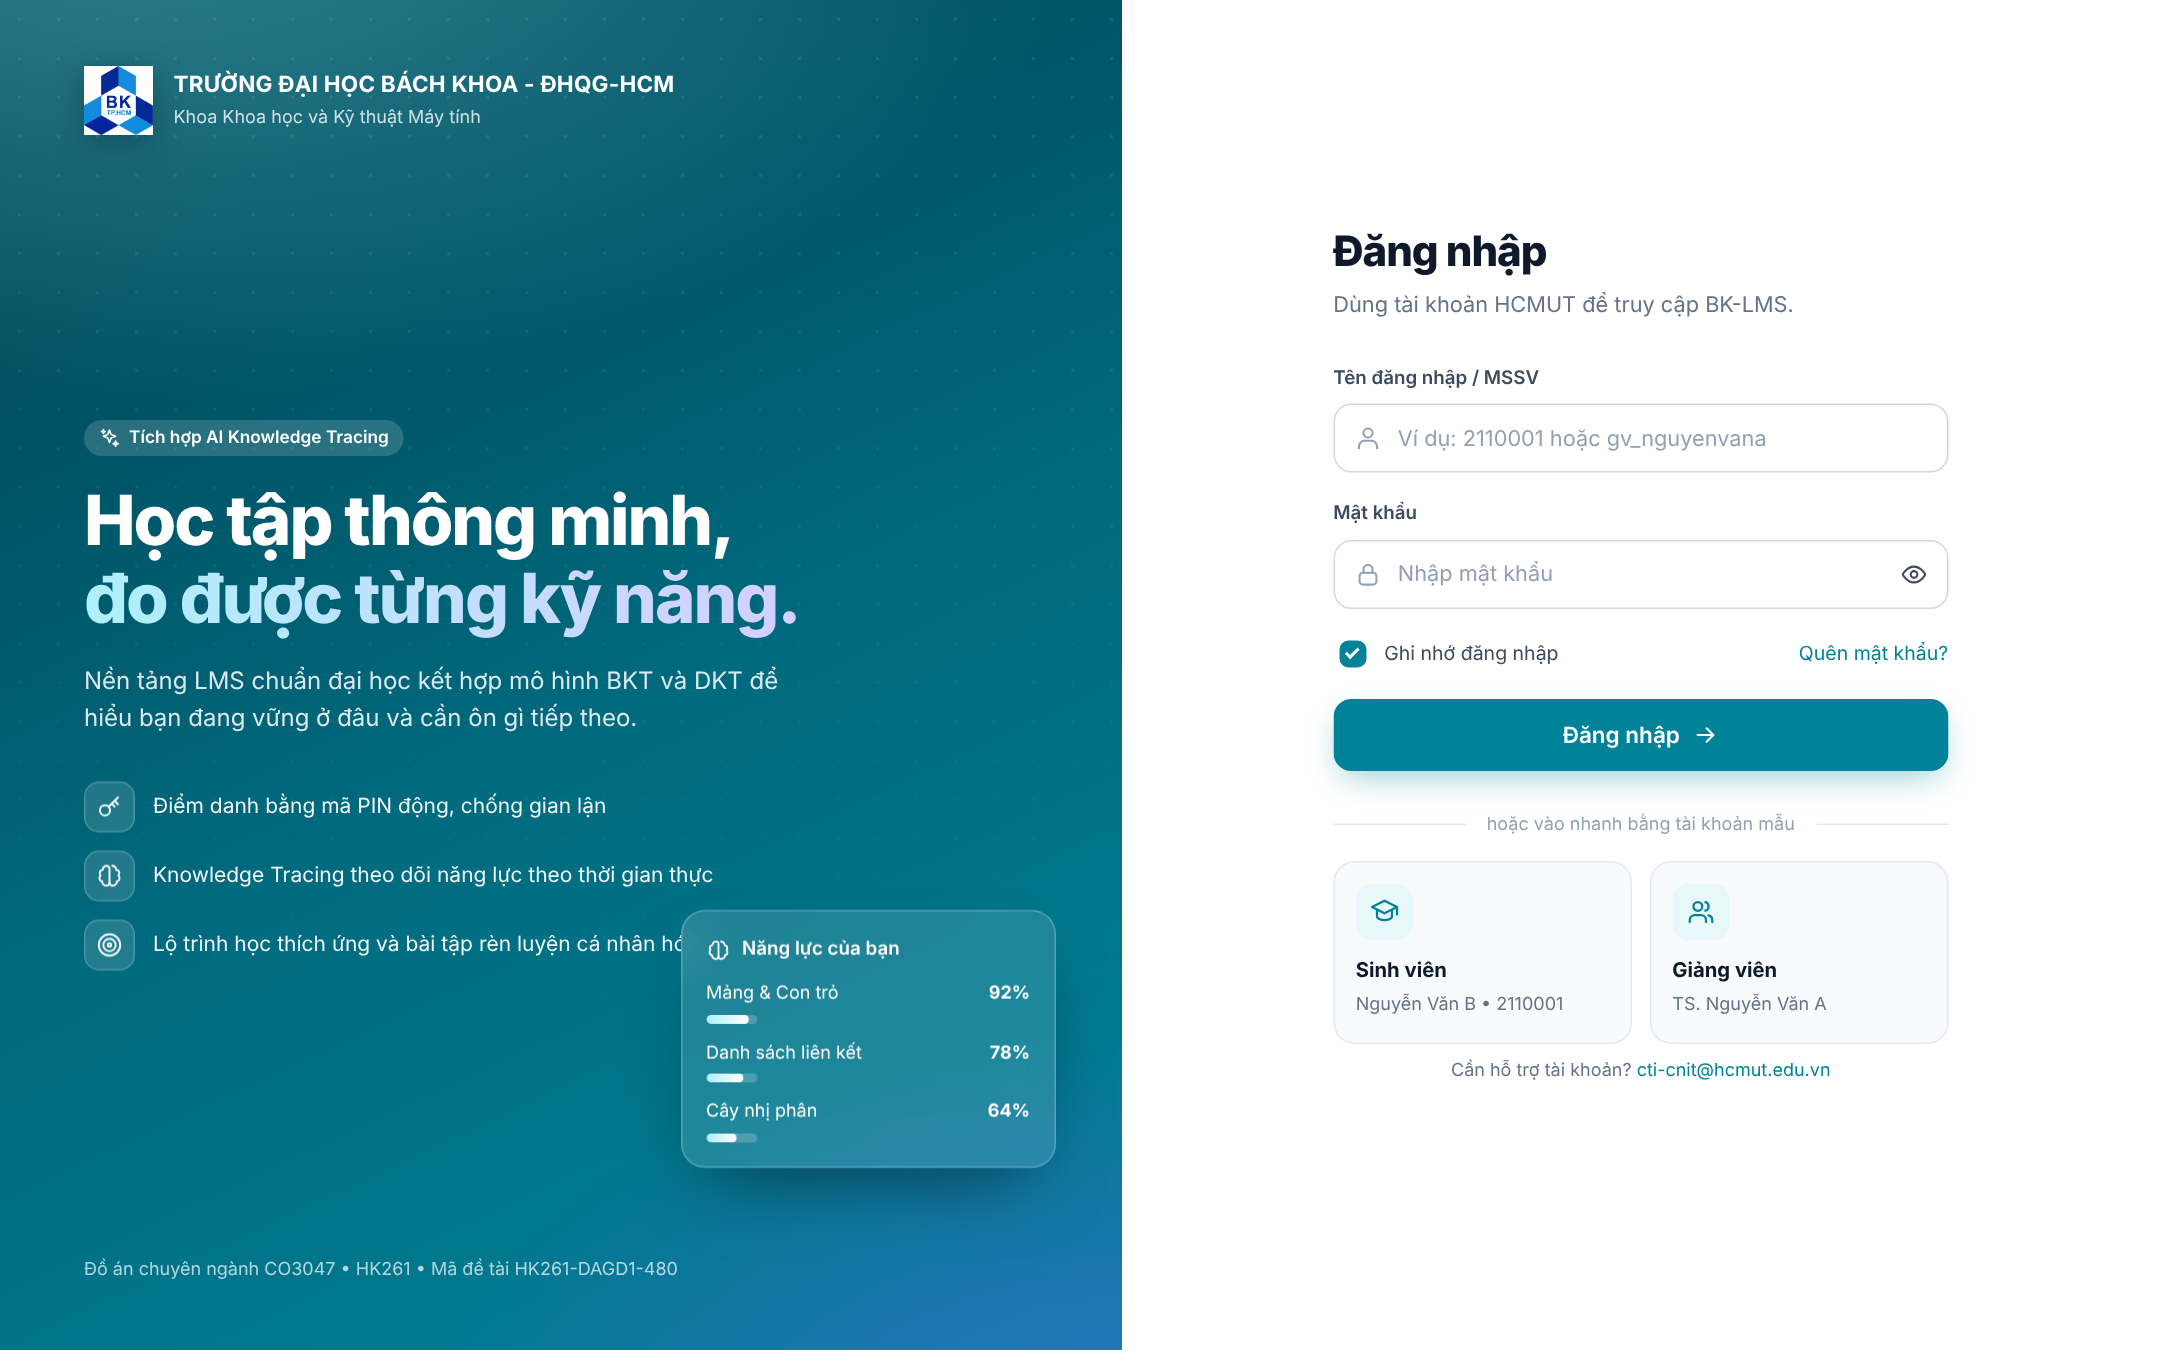
\includegraphics[width=0.6\linewidth]{images/login.png}
\caption{Login page in the style of HCMUT CAS, with separate lecturer and student entries}
\label{fig:login}
\end{figure}

\begin{figure}[H]
\centering
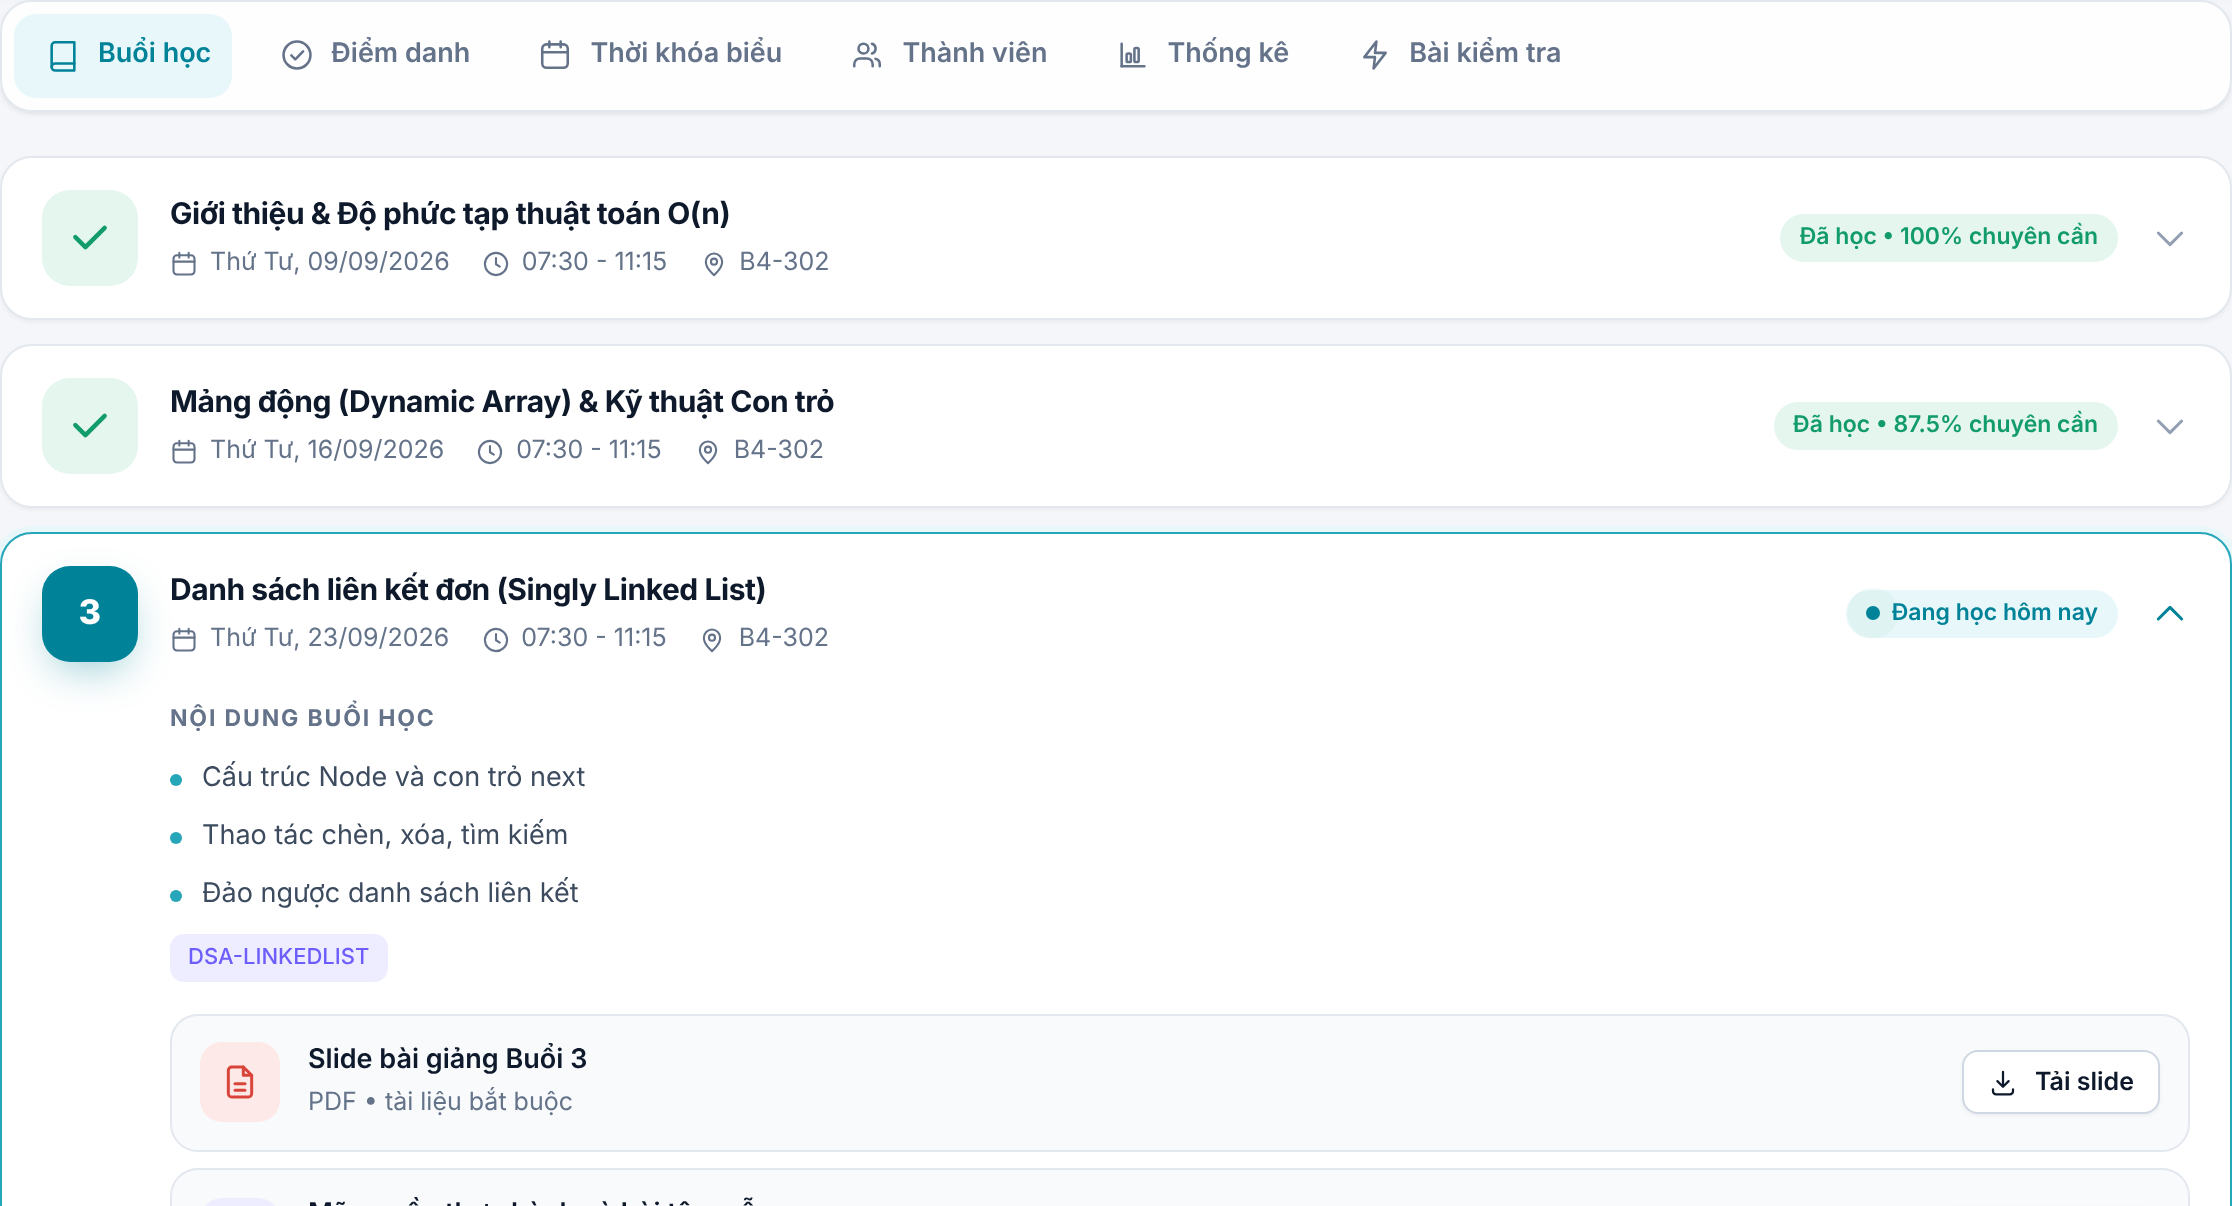
\includegraphics[width=0.82\linewidth]{images/c_sessions.png}
\caption{Course page: the fifteen sessions of CO2003 with their materials}
\label{fig:sessions}
\end{figure}

\begin{figure}[H]
\centering
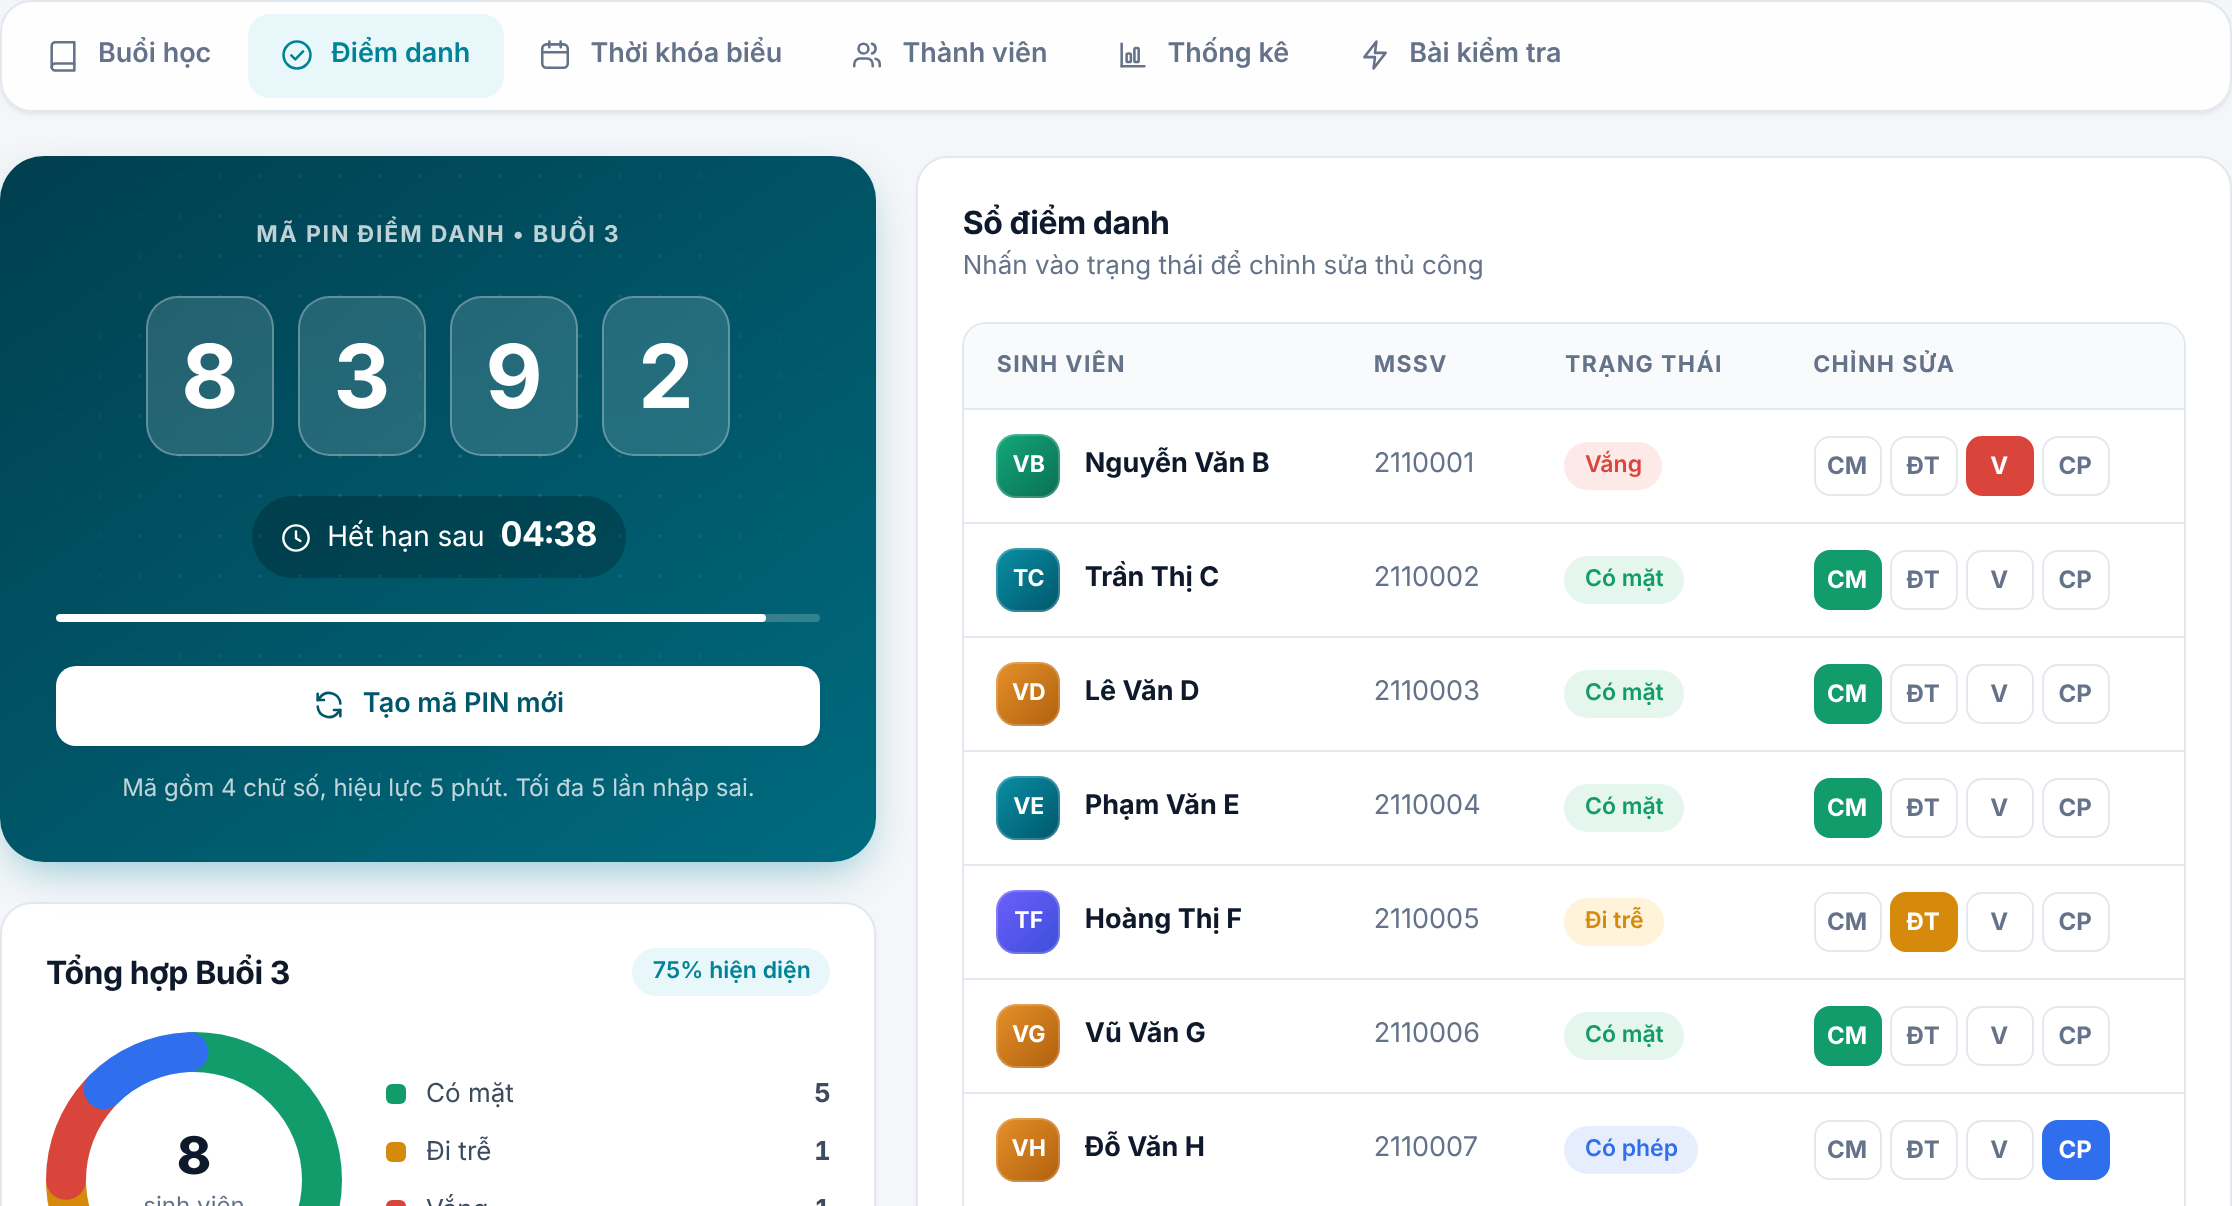
\includegraphics[width=0.82\linewidth]{images/c_attendance.png}
\caption{Attendance tab: the PIN window opened by the lecturer, with countdown and class list}
\label{fig:attendance}
\end{figure}

\begin{figure}[H]
\centering
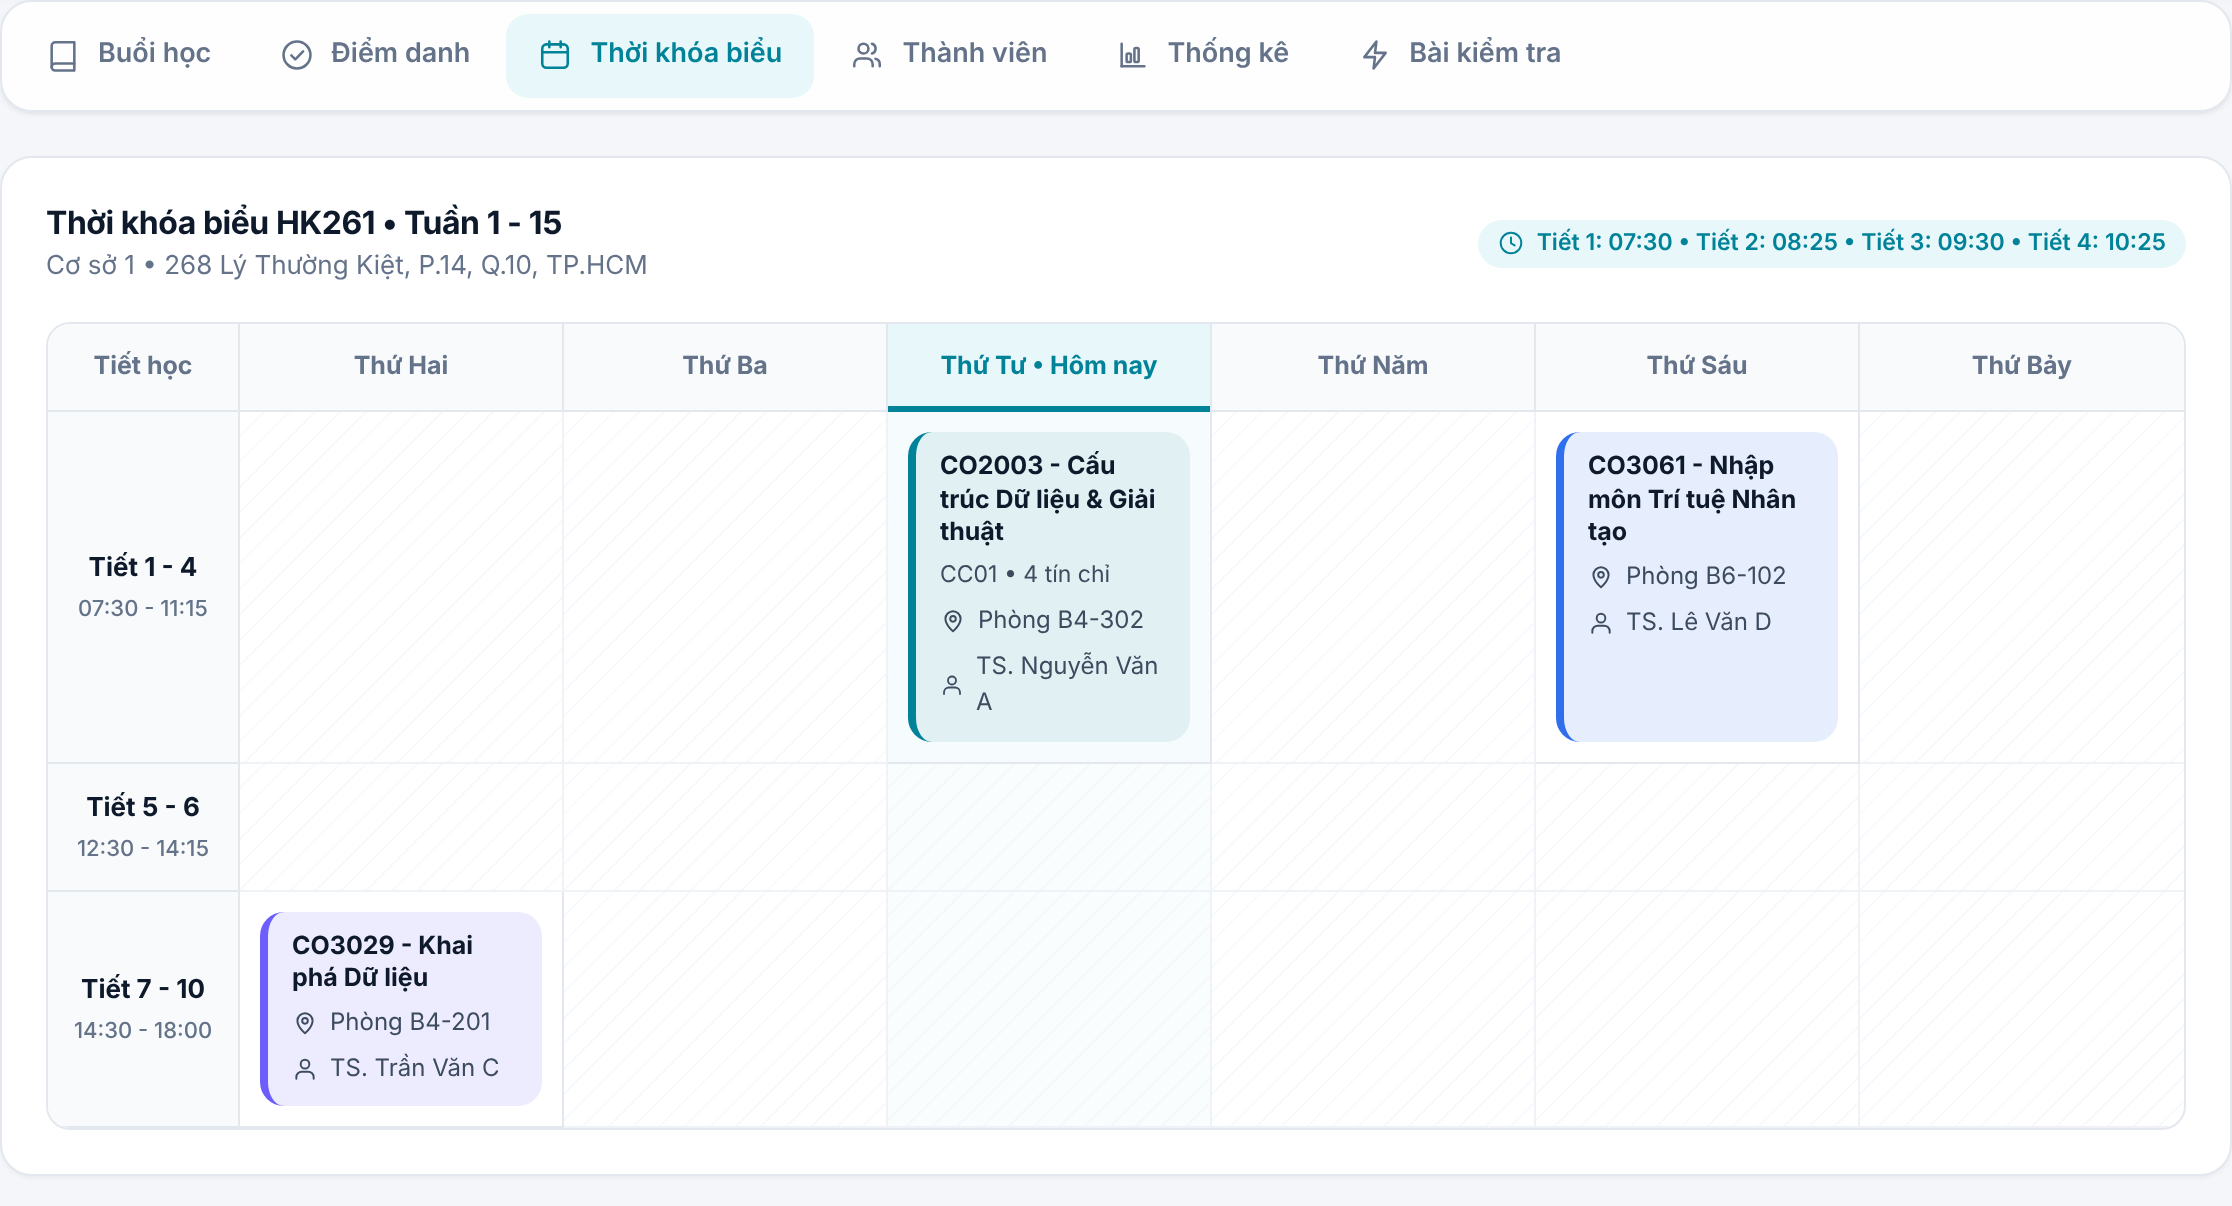
\includegraphics[width=0.82\linewidth]{images/c_timetable.png}
\caption{Weekly timetable with the current session highlighted}
\label{fig:timetable}
\end{figure}

\begin{figure}[H]
\centering
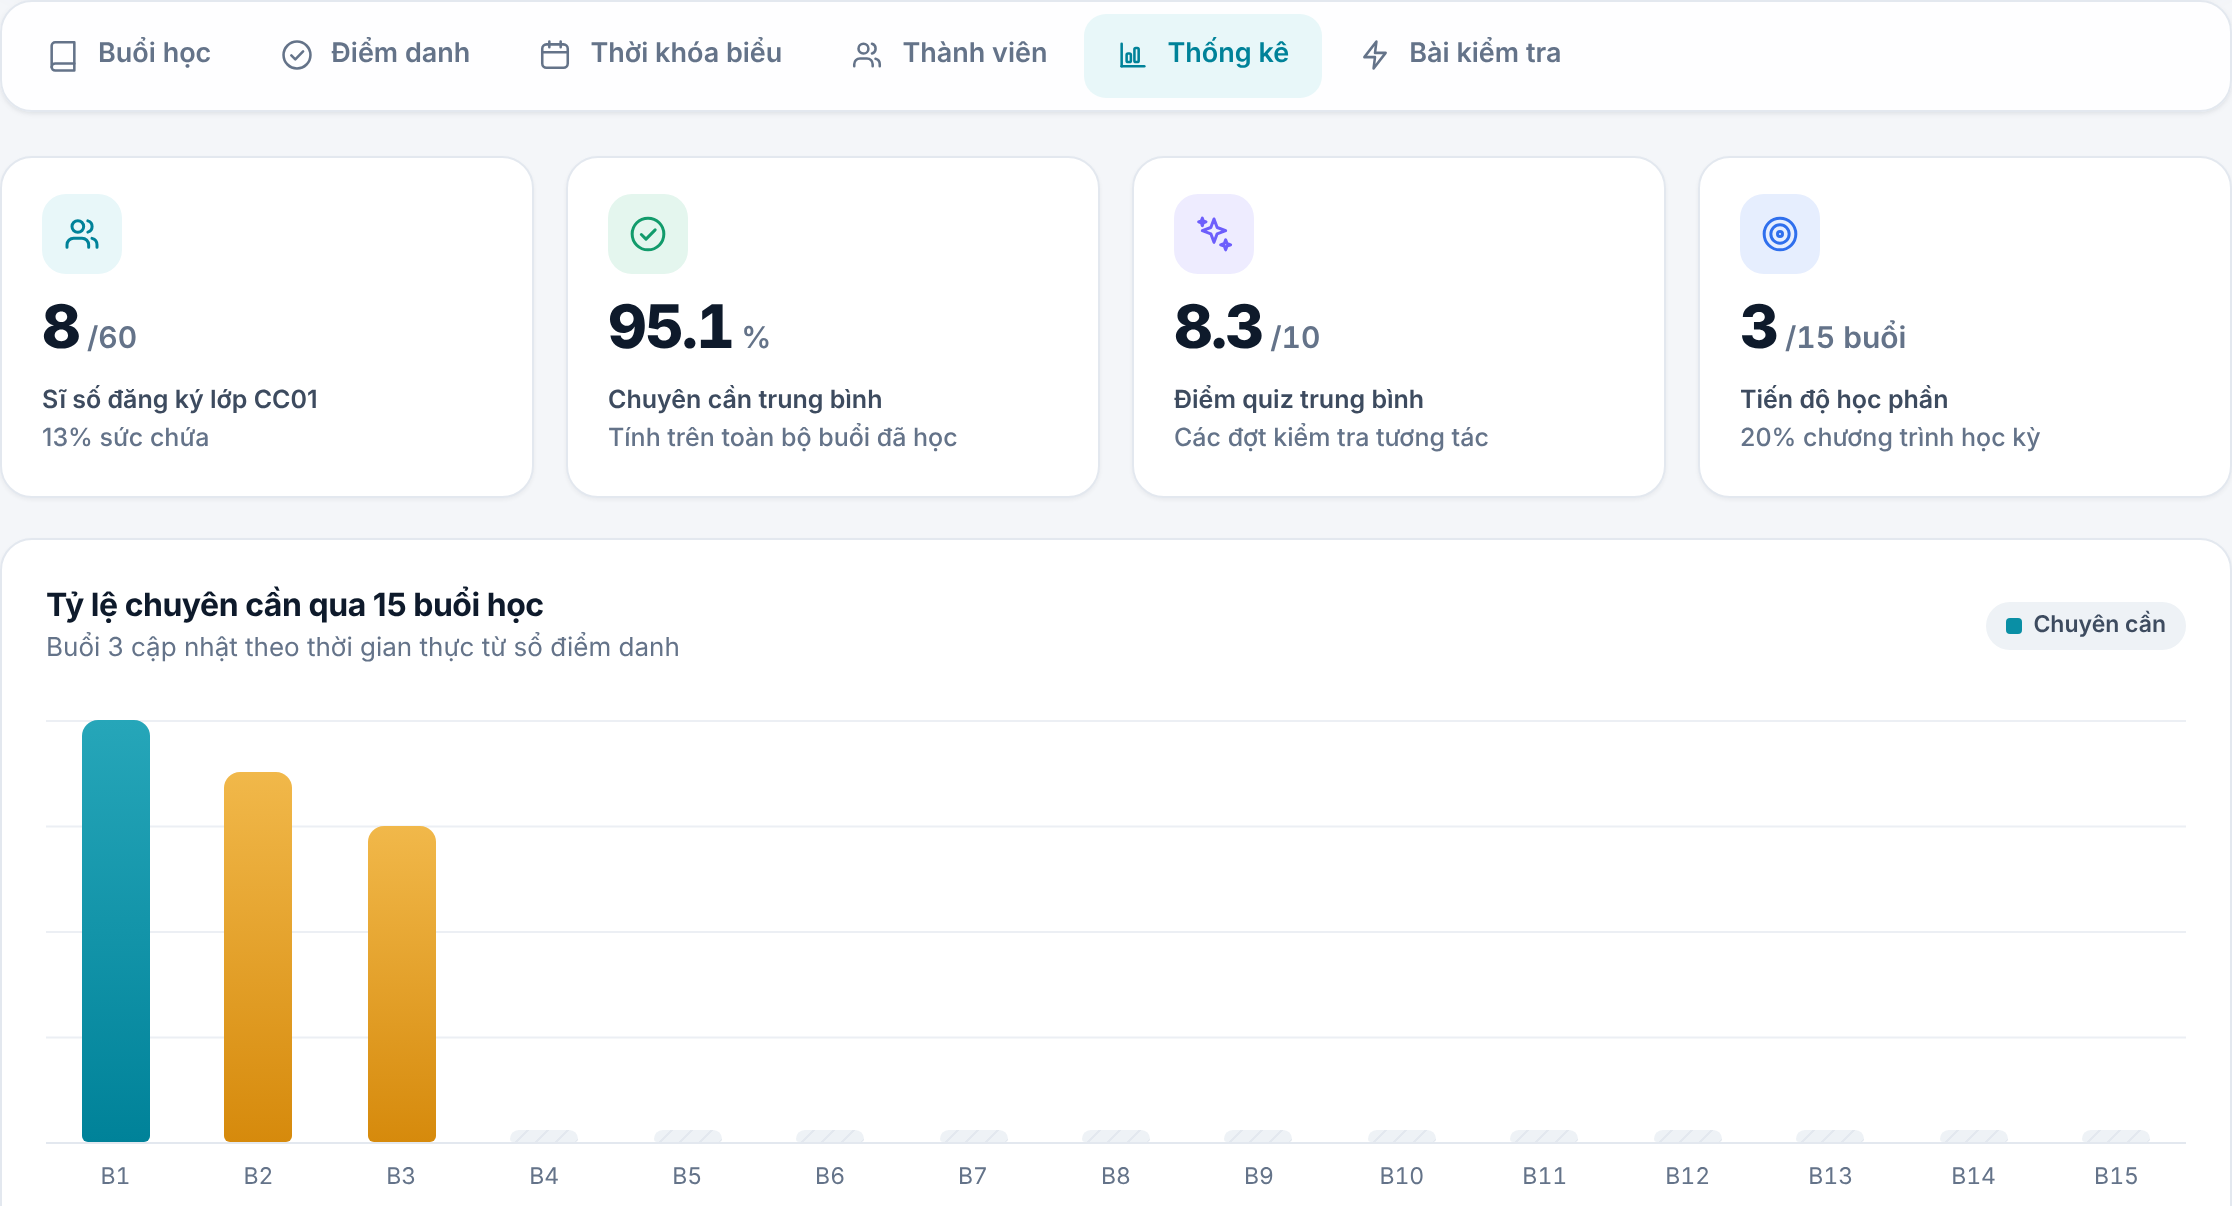
\includegraphics[width=0.82\linewidth]{images/c_stats.png}
\caption{Statistics tab: enrollment against capacity, participation per session and rate per student}
\label{fig:stats}
\end{figure}

\subsubsection{Authentication in the Prototype}

The login page separates the two roles from the first screen instead of offering a role switch on the navigation bar, which a real system would not have. Sample accounts allow the demonstration to start with one click. At the time of writing, the prototype uses data stored in the front end for its demonstration; connecting each page to the REST API is the first task of the next semester (Section~\ref{ch:plan}). We state this clearly so that the reader does not confuse the demonstration data with data coming from the database.

\subsection{Pilot Dataset: CO2003}
\label{sec:dataset}

To test the design with realistic content, the team prepared the dataset of a pilot course. The course is \emph{Data Structures and Algorithms} (CO2003, 4 credits), class CC01 of semester HK261. The dataset is stored as Markdown and JSON in the repository and can be loaded into the tables \code{course_sessions}, \code{skills}, \code{quizzes} and \code{questions}.

\subsubsection{Fifteen-Session Outline}

Table~\ref{tab:sessions} shows the outline. Each session has a title, one main skill, and a learning objective. The date of each session is computed from the start date of the semester when the data are loaded.

\begin{table}[H]
\centering
\caption{Fifteen-session outline of CO2003}
\label{tab:sessions}
\begin{tblr}{colspec={Q[c,0.9cm]Q[l,4.2cm]Q[l,3.3cm]X[l]}, row{1}={font=\bfseries}, hline{1,Z}={0.8pt}, hline{2}={0.4pt}, rowsep=2pt, rows={font=\small}}
No. & Title & Skill & Objective\\
1 & Course introduction and C++ review & \code{DSA-ARRAY} & Course goals; basic C++ and pointers\\
2 & Arrays, pointers, dynamic allocation & \code{DSA-ARRAY} & Allocate and free dynamic memory\\
3 & Algorithm complexity analysis & \code{DSA-COMPLEXITY} & Compute Big-O of simple code\\
4 & Singly linked lists & \code{DSA-LINKEDLIST} & Insert, delete, search\\
5 & Doubly and circular linked lists & \code{DSA-LINKEDLIST} & Distinguish and implement variants\\
6 & Stack & \code{DSA-STACK} & LIFO; balanced parentheses; postfix\\
7 & Queue & \code{DSA-QUEUE} & FIFO; circular queue\\
8 & Recursion & \code{DSA-RECURSION} & Base case and recursive step; cost\\
9 & Sorting & \code{DSA-SORT} & Selection, insertion, merge, quick\\
10 & Trees and binary trees & \code{DSA-TREE} & Terminology; traversals\\
11 & Binary search trees & \code{DSA-TREE} & Insert, delete, search; degenerate case\\
12 & AVL trees & \code{DSA-TREE} & Balance condition; rotations\\
13 & Heaps and priority queues & \code{DSA-HEAP} & Array heap; heap sort\\
14 & Graphs & \code{DSA-GRAPH} & Representations; BFS and DFS\\
15 & Hash tables and review & \code{DSA-HASH} & Hash functions; collisions; course review\\
\end{tblr}
\end{table}

\subsubsection{Skills and Question Bank}

The bank has 40 multiple-choice questions with four options, one correct option, a difficulty level (easy, medium, hard), a session number and a one-sentence explanation. Each question is labeled with exactly one of eleven skills. The correct answers are shuffled over the four positions to avoid a bias toward one letter. Table~\ref{tab:skills} shows the distribution.

\begin{table}[H]
\centering
\caption{Skills (knowledge components) and number of questions}
\label{tab:skills}
\begin{tblr}{colspec={Q[l,4cm]X[l]Q[r,2.2cm]}, row{1}={font=\bfseries}, hline{1,Z}={0.8pt}, hline{2}={0.4pt}, rowsep=2pt}
Skill code & Content & Questions\\
\code{DSA-ARRAY} & Arrays and pointers & 5\\
\code{DSA-COMPLEXITY} & Algorithm complexity & 1\\
\code{DSA-LINKEDLIST} & Linked lists & 6\\
\code{DSA-STACK} & Stack & 4\\
\code{DSA-QUEUE} & Queue & 3\\
\code{DSA-RECURSION} & Recursion & 1\\
\code{DSA-SORT} & Sorting & 2\\
\code{DSA-TREE} & Binary trees, BST, AVL & 8\\
\code{DSA-HEAP} & Heap & 2\\
\code{DSA-GRAPH} & Graphs & 5\\
\code{DSA-HASH} & Hash tables & 3\\
\textbf{Total} & & \textbf{40}\\
\end{tblr}
\end{table}

\paragraph{Example.} Question DSA-Q09 (session 4, skill \code{DSA-LINKEDLIST}, medium): ``To delete the node right after node $p$ (where $p\rightarrow next$ is not NULL), the correct approach is?'' The correct option is: save $q = p\rightarrow next$, set $p\rightarrow next = q\rightarrow next$, then free $q$. The explanation states that the node to delete must be saved before relinking, otherwise the reference is lost.

\paragraph{Remarks on the dataset.} The distribution is not uniform: complexity and recursion have one question each, which is too few for any statistical use. Expanding the bank to at least 3--5 questions per skill is part of the plan for HK262. The sample schedule in the dataset (Tuesday, periods 2--4, room H6-302) is a sample value and differs from the demonstration data of the prototype; both are replaced by the real timetable when the class is registered.

\subsection{Traceability: From Requirements to Code}

Table~\ref{tab:trace} shows, for every functional requirement, where it is implemented and its status at the date of this report. ``API'' means the endpoint exists in the back end; ``UI'' means a screen exists in the prototype.

\begin{table}[H]
\centering
\caption{Requirements traceability and implementation status (November 2026)}
\label{tab:trace}
\begin{tblr}{colspec={Q[l,1.2cm]X[l]Q[l,2.0cm]Q[l,2.0cm]}, row{1}={font=\bfseries}, hline{1,Z}={0.8pt}, hline{2}={0.4pt}, rowsep=2pt, rows={font=\small}}
ID & Where implemented & API & UI\\
FR1 & \code{/api/auth/*}, login page & Yes & Yes\\
FR2 & \code{/api/schedule}, course cards & Yes & Yes\\
FR3 & \code{/api/classes/:id/enroll}, trigger & Yes & Partial\\
FR4 & \code{/sessions}, \code{/sessions/bulk} & Create only & Yes\\
FR5 & \code{CHECK}/\code{UNIQUE} (number, time range); room-conflict check is not implemented yet & Partial & Partial\\
FR6 & \code{/api/schedule}, timetable tab & Yes & Yes\\
FR7 & \code{session_materials}, sessions tab & Read & Yes\\
FR8 & \code{/attendance/open} & Yes & Yes\\
FR9 & \code{/attendance/check-in} & Yes & Yes\\
FR10 & Check-in transaction & Yes & Yes\\
FR11 & \code{/attendance/close}; manual marking & Close only & Yes\\
FR12 & \code{/attendance/summary} & Yes & Yes\\
FR13 & \code{/quizzes/:id/submit} & Yes & Yes\\
FR14 & Question creation & No & No\\
FR15 & Theme variables & --- & Yes\\
\end{tblr}
\end{table}

\noindent\textit{Note.} ``UI = Yes'' means that a screen exists in the prototype. The screens currently use demonstration data kept in the front end and are not yet connected to the REST API; the connection is the first task of Section~\ref{ch:plan}.
